\section{Host-Level Security Isolation}
\label{sec:linux:security}

\issuedone{1.1.d}{describe the security isolation story for Linux hosts}
\graphene{} separates OS features from security isolation by making the latter a duty of the host.
This section explains the Linux PAL design for isolating mutually untrusting applications, with a reduce interface to attack the host kernel.
This section starts with stating the motivation and threat model of the security isolation mechanism,
followed by the technical discussion of implementation
in a Linux host.



\subsection{Motivation and threat model}

\graphene{} ensures that mutually untrusting applications 
cannot interfere with each other, providing security isolation
comparable to running in separate VMs.
\graphene{} reduces the attack surface exposed to applications
by restricting access to the host kernel ABI 
and prevents access to unauthorized system calls, files, byte streams,
and network addresses with a \emph{reference monitor}.
%The host kernel ABI exported by the \pal{} heavily 
%limits the ability of a \graphene{} application to interact with the rest of the system;
%any external interactions are further mediated by a reference monitor.
%Unlike a typical Linux system, \graphene{} applications cannot interact with shared 
%system daemons or other shared system resources.
%As a result, \graphene{} enforces security isolation similar to running applications in separate VMs---even
%applications that span multiple processes.
\graphene{} contributes a multi-process security model 
based on the abstraction of a \emph{sandbox},
or a set of mutually trusting picoprocesses.
The reference monitor permits picoprocesses within the same sandbox
to communicate and exchange RPC messages, but disallows cross-sandbox communication.
The current work focuses on all-or-nothing security isolation, although we expect
this design could support
controlled communication among mutually untrusting \liboses{}
in future work.

The only kernel-level sharing abstractions the reference monitor must mediate
are files, network sockets, and RPC streams
--- all other allowed kernel ABIs
modify only local \picoproc{} state.
%Thus, the reference monitor need only mediate file access, socket and RPC stream creation.
%an unprivileged daemon
%as well as extensions to the App\-Armor LSM~\cite{apparmor},
%which checks file and socket policies in the kernel.
%, reducing context switching overhead
%and the risk of race conditions~\cite{garfinkel03traps}.
In order for the reference monitor to restrict file access, socket and RPC stream creation,
each application includes a \emph{manifest file}~\cite{hunt07rethink},
which describes a {\tt chroot}-like, restricted view of the local 
file system (similar to Plan 9's unioned file system views~\cite{pike90plan9}),
%including read-only shared files,
as well as \emph{iptables}-style~\cite{iptablesman} network restrictions.
%%% To facilitate sharing read-only libraries,
%%% a manifest may specify a file system view which 
%%% combines several different sub-directories of the local file system,
%%% and can prevent writing to files or directories.


%The \graphene{} reference monitor on a Linux host
%is implemented using {\tt ioctl} system call to a special device {\tt /dev/graphene}.
%A picoprocess is restricted by seccomp filter~\cite{seccomp} to use any {\tt open} or socket {\tt connect} and {\tt bind} system calls.
%It must use the \graphene{} special device to open or create streams,
%so the file paths or network addresses can be checked against the sandbox rules.
%The kernel module as the driver of the \graphene{} special device can coexist with any LSM such as \emph{AppArmor} or \emph{SELinux}.


\fixme{Explain with a figure.}
When a new picoprocess is launched by the reference monitor, it begins execution in 
a new sandbox.  
Child picoprocesses may either inherit their parent's sandbox, 
or can be started in a separate sandbox
--- specified by a flag to the picoprocess creation ABI.
A parent may specify a subset of its own file system view 
when creating a child, but may not request access to new regions of the 
host file system. 
%The restrictive policy enforced on the child will be written in a new manifest file generated by the parent, and the policy will be checked by the reference monitor.
The child may also issue an {\tt ioctl} call to 
dynamically detach from the parent's sandbox. The reference monitor prevents byte stream creation 
across sandboxes.
%among picoprocesses
%that are not in the same sandbox.
%and restricts external connections to remote URIs according to firewall rules in the manifest.
When a process detaches from a sandbox --- effectively splitting the sandbox ---
the reference monitor closes
any byte streams that could bridge the two sandboxes.

\paragraph{Threat models.}
We assume  a trustworthy host OS and reference monitor,
which mediates all system calls with effects outside of a picoprocess's address space,
such as file {\tt open} or network socket {\tt bind} or {\tt connect}.
We assume that picoprocesses inside the same sandbox trust each other and that all untrusted code runs in sandboxed picoprocesses.
We assume the adversary can run arbitrary code inside of
one or more picoprocesses within one or more sandboxes.
The adversary can control all code in its
picoprocesses, including {\tt libLinux} and the \pal{}. 
%We also assume a trusted reference monitor process running on the host kernel that 
%launches \graphene{} applications and mediates all system calls with external effects,\fixmedp{define precisely}

\graphene{} ensures that %The key security property the \graphene{} design upholds is that 
the adversary cannot interfere with any victim picoprocesses
in a separate sandbox.  
The \graphene{} sandbox design ensures strict isolation: 
if the only shared kernel abstractions are byte streams and files, 
and the reference monitor ensures
there is no writable intersection between sandboxes,
the adversary cannot interfere with any victim picoprocess.


%%% The only processes allowed to run as standard kernel processes (non-\graphene{}) 
%%% are the reference monitor and
%%% system administration utilities that need more kernel interfaces than the \pal{} ABI provides.
%%% Ensuring that a collaborating picoprocess correctly implements
%%% some function (such as receiving a signal),
%%% as well as preventing exploitation of vulnerabilities in picoprocesses
%%% are beyond the scope of this work.

\graphene{} reduces the system attack surface of the host, but does not change the size of its
trusted computing base; however, reducing the effective system call table
size of a picoprocess does facilitate adoption of a smaller host kernel,
which we leave for future work.

\subsection{System call restriction}

Unmodified Linux applications run on \graphene{} by issuing 
system calls as library calls to {\tt libLinux}.
Application calls are serviced by {\tt libLinux}-internal data structures
or \pal{} calls.
The \pal{} is implemented using \hostsyscallnum{} host system calls.
The host OS must block any 
native system call that 
does not appear in the \pal{} source code.
Any allowed system call with external effects is checked by 
the reference monitor.
 
%% dp: Meh
%%% Any picoprocess implementation 
%%% must restrict access to the host system call table,
%%% generally by blocking system calls in the host kernel~\cite{porter11drawbridge}
%%% or using {\tt ptrace}~\cite{xax}.


%The \pal{} is a host-provided library which implements \palcalls{} generic kernel ABIs,
%implemented using 
%These native system calls include {\tt ioctl} with 5 opcodes exclusively used by \graphene{} kernel extensions.

%This section describes how we adapt recent Linux sandboxing techniques 
%to \graphene{}.


%all allowed system calls with potentially external effects.

%%% For instance, an attempt to open a file will be checked by the reference monitor
%%% to see if the file is included in the sandbox definition, specified in the manifest
%%% with required permissions.
%%% Once the file handle is open, the \pal{} is then allowed to issue an {\tt mmap} or {\tt read}
%%% on the handle, as this operation can only affect the picoprocess address space
%%% or  file, which was already checked.

%Because the \pal{} is in the same address space as the application code, it is not
%trusted to enforce any security policies, and our threat model assumes that
%the \pal{} can be compromised by the adversary.
%Thus, the host kernel 
%only permits system calls that appear in the \pal{}'s source code and, through the reference monitor, further inspects calls that can have external effects.

\begin{figure}[t!]
\centering
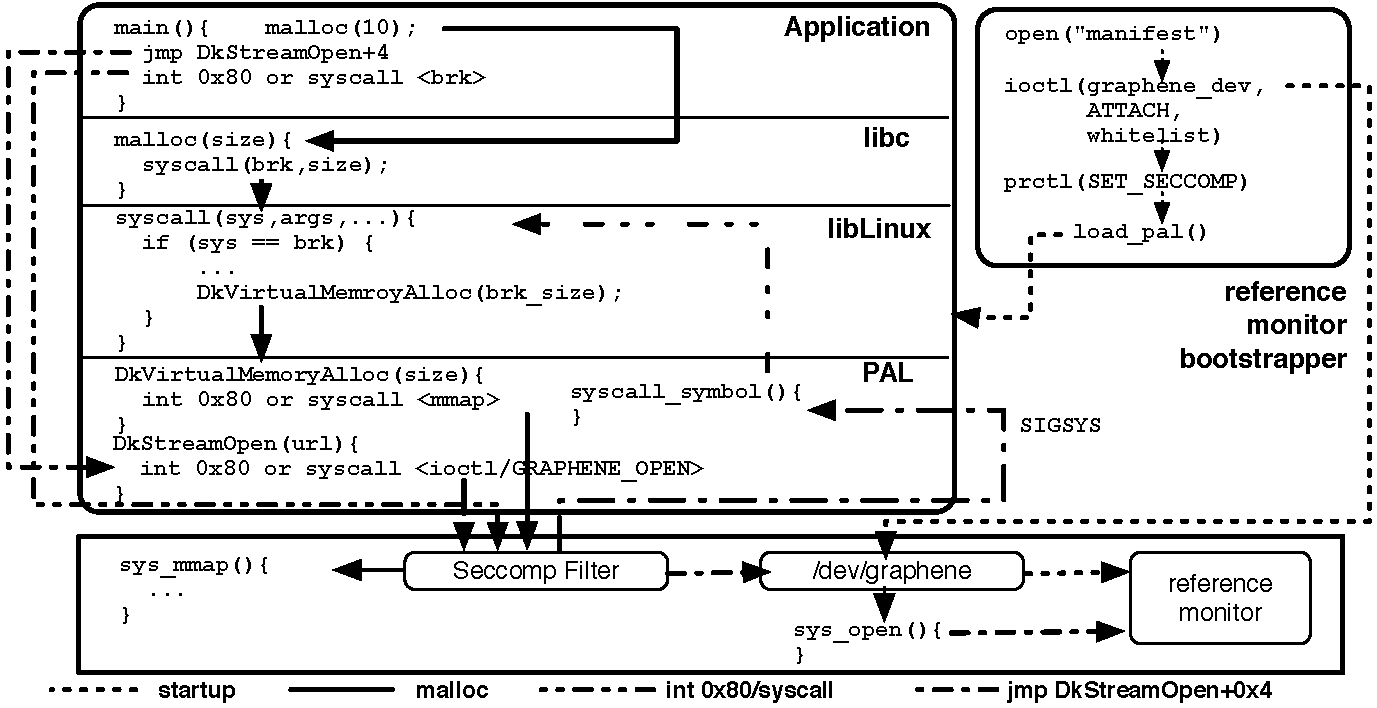
\includegraphics[width=\linewidth]{syscall-restriction.pdf}
\footnotesize
\caption[System call restriction approach in sysname{}]
{System call restriction approach. The reference monitor loads policies into the LSM at startup.  A \graphene{} application requests OS services in three different ways. 
In the normal case (first line of {\tt main}), {\tt malloc} is invoked causing the invocation of {\tt brk} ({\tt libLinux}) and {\tt mmap} in the \pal{}. In the second line, the application jumps to an address in \pal{}, which is permissible.
Files are accessed through {\tt ioctl} to {\tt /dev/graphene} and checked by reference monitor.
The third line invokes {\tt brk} with an {\tt int} instruction, which is redirected to the {\tt libLinux} function.}
\label{fig:graphene:syscall-restriction}
\end{figure}



\issue{1.3.d}{extend the discussion of SECCOMP filter}
\graphene{} restricts the host system call table 
using seccomp~\cite{seccomp}, introduced in Linux 2.6.12.
% a recent Linux system call filtering mechanism, called 
Seccomp allows a process to create an immutable Berkeley Packet Filter (BPF) program
that specifies allowed system calls, as well as creates {\tt ptrace} 
events on certain system calls.
The filter can also filter scalar argument values,
such as only permitting specific {\tt ioctl} opcodes.
%The BPF grammar is rich enough to filter system calls by 
%This feature is particularly salient in the case of {\tt ioctl},
%where the \pal{} uses 5 out of over 400 opcodes for our bulk IPC module and sandbox creation;
%our BPF rules will block any other {\tt ioctl} opcode.
If a system call is rejected, the \pal{} will receive a {\tt SIGSYS} signal,
and can either terminate the application or redirect the 
call to {\tt libLinux}.
Seccomp filters cannot be overridden by any picoprocess,
and are always inherited.
% by all descendant processes.
The current \graphene{} filter is 79 lines 
of straightforward BPF macros.  In our experience, adding more precise argument checks
has not significantly changed performance.

%Seccomp filters are installed using the {\tt prctl} system call;
%blocking {\tt prctl} in a seccomp filter prevents further changes to the filter.

Unfortunately, the logic to check for allowed paths network addresses cannot be implemented 
as a seccomp rule, because it involves reading user memory of unknown sizes. 
In order to avoid the overhead of trapping to the reference monitor on 
every use of {\tt open}, {\tt stat}, {\tt bind} or {\tt connect} system calls, we instead 
force picoprocess to only use {\tt ioctl} system call to \graphene{} special device ({\tt /dev/graphene}) as alternative interface these system calls. Direct access to these system calls are banned by seccomp filter.
%extend AppArmor~\cite{apparmor} 
%to enforce file system isolation in the kernel.

In order to reduce the impact of bugs in the reference monitor,
the reference monitor itself runs with a seccomp filter,
blocking unexpected system calls.

\paragraph{Static Binaries.} 
For compatibility with statically linked binaries, which 
compile in system call instructions,
we leverage seccomp to redirect these calls 
back to {\tt libLinux}.  
For system calls that could also be issued by the \pal{},
we augment our BPF rules with program counter-based filters.
In other words, an {\tt open} system call with a return PC address inside the \pal{} 
will be sent to the reference monitor for further inspection;
an {\tt open} system call with any other return PC address generates 
a {\tt SIGSYS} and is ultimately relayed back to {\tt libLinux}.
Thus, {\tt libLinux} can catch and differentiate application-issued system calls
from those that could also be issued by the \pal{}.
We hasten to note this feature is only for backward compatibility,
not security. 


\subsection{Sandboxing untrusted applications}


\begin{comment}
We hasten to note that program counter filtering
is only provided for backwards compatibility, not security.
An attacker can compromise the \pal{}, so system policies are enforced
externally by the reference monitor.


Dynamically redirecting system calls to {\tt libLinux} is 
less efficient than dynamically linking against
the \graphene{} libc or statically compiling {\tt libLinux} into the application.
The overhead of dynamic redirection comes from 
transferring control to the kernel, then back to 
the \pal{}, and then to {\tt libLinux}.
We leave exploration of more efficient alternatives for future work,
such as redirecting the hardware system call table to {\tt libLinux}
on a host system like Dune~\cite{belay12dune},
or dynamically rewriting parts of the static binary~\cite{hunt99detours}.
\end{comment}

\paragraph{Example.}
Figure~\ref{fig:graphene:syscall-restriction} illustrates three possible situations. 
%% An unmodified Linux application is dynamically linked against the 
%% \graphene{} {\tt libc}, 
%% which then dynamically links its system calls from {\tt libLinux},
%% which in turn links in the host kernel ABI from the \pal{}.
%% The application requests OS functionality in three ways.
An unmodified application first invokes the {\tt libc} function {\tt malloc}, which issues 
a {\tt brk} system call to {\tt libLinux}, which requests memory 
from the host via a {\tt Dk\-Virtual\-Memory\-Alloc} \pal{} call,
which ultimately issues an {\tt mmap} host system call.
The {\tt mmap} host system call is allowed by seccomp because it only 
affects the picoprocess's address space.
The second line of the application jumps to the \pal{} instruction that issues
an {\tt open} system call.
From a security perspective, this is permissible,
as it is isomorphic to \pal{} functionality.
In practice, this could cause
corruption of {\tt libLinux} or application data structures,
but the only harm is to the application itself. 
Because this system call involves the file system, the reference monitor LSM first checks if the file to be opened is included in the sandbox definition (manifest) before allowing  the {\tt open} system call in the kernel.  
Finally, the application uses inline assembly to issue a {\tt brk} system call;
%in an attempt to obtain I/O port privilege; 
because this system call was not issued by the \pal{},
seccomp will redirect this call back to the \pal{},
which then calls the {\tt libLinux} implementation.

\paragraph{Process-specific Isolation.} 
Sandbox creation in \graphene{} can provide
more options than virtualization, to reflect the security policy of applications at any timing,
in the granularity of picoprocess. 
A picoprocess can voluntarily detach itself from the current sandbox, dropping its privileges,
after finishing security-sensitive operations.
If a picoprocess decides one of its children is not trustworthy, it may also start the child under a restricted manifest,
or promptly shut down RPC streams to stop sharing OS states.
The picoprocess that moves to a separate sandbox will have a restrictive view of the filesystem, and no coordination with the previous sandboxes.
In section~\ref{sec:graphene:eval}, we describe an experiment that improves security isolation of Apache web server without sacrificing functionality.

\paragraph{Reference monitor.}
The reference monitor is a trusted process that runs on the host system.
\graphene{} applications are launched by the reference monitor,
which instantiates the seccomp filter and traces all children
to check host system calls that could have external effects.
The reference monitor interposes using ptrace events, 
which can be raised for specific system calls by seccomp.
We ensure that all processes created within a sandbox are traced
by setting the {\tt PTRACE\_O\_TRACESECCOMP} option on all newly created picoprocesses
in the sandbox.

%% from bpjain:
% We have to set the option PTRACE\_O\_TRACESECCOMP on new children
% using ptrace(PTRACE\_SETOPTIONS) and we get the event as
% PTRACE\_EVENT\_SECCOMP whenever a syscall that is Traced is called.
% It happens before the grandchild starts running. We get the
% notification of creation of grandchildren by setting ptrace option
% PTRACE\_O\_TRACECLONE on the child(i.e., parent of grandchild).  I
% need to monitor every fork/clone (only clone since pal only calls
% clone). I get this event even if fork/clone is just allowed.  And
% the event that arrives on clone/fork is completely different from
% seccomp event. Thats a ptrace event too.. but we get
% PTRACE\_EVENT\_CLONE whenever a clone is done by a child on which
% PTRACE\_O\_TRACECLONE option was set.

Each application includes a \emph{manifest file}, which specifies restrictions,
including network firewall rules and subsets of the host file system sandboxed
applications are permitted to access.  The reference monitor enforces these
rules by interposing on all system calls involving file paths or remote network addresses.
%\fixmedp{Revise if we can do something smarter; 2x check implementation status before submission}.

%% dp Sadface :(
\paragraph{Privilege.~} 
Although the reference monitor is trusted, it does not run 
with administrative privilege.
Linux 3.5, which we use as our host kernel, 
introduced the {\tt NO\_NEW\_PRIVS} bit, which permits
a non-privileged process to impose sandboxing restrictions on a child.
%Ubuntu back-ported this feature to Linux 3.2, which we use as our host kernel.
This flag prevents a process from acquiring root privilege, % (e.g., via executing a {\tt setuid} binary),
is inherited by all descendant processes,
and cannot be disabled.

\paragraph{Creating New Sandboxes.~} We add a \pal{} call which
permits a picoprocess to request that it be moved into a new sandbox.
This call, as well as file system path checks, are implemented
as extensions to the  AppArmor LSM~\cite{apparmor}.
%We modify \sandboxmodlines{} lines in the
%to implement this call,
The new sandbox call closes any open stream handles that cross sandbox boundaries;
mediate path lookups;
and create a new broadcast stream for multi-process
 coordination (\S\ref{sec:graphene:namespaces:blocks}).
%The reference monitor also interposes on this call so that it can 
%mediate future stream creation.

To securely apply seccomp filtering we leveraged the fact that all
\graphene{} processes have the same parent and also the new
{\tt NO\_NEW\_PRIVS} bit introduced for Linux processes starting kernel
version 3.5. This bit can be set by any process, is inherited across
{\tt fork}, {\tt clone}, and {\tt execve}, and cannot be unset by
children processes. Thus, we set the {\tt NO\_NEW\_PRIVS} bit in the initial
\graphene{} process and apply seccomp filters allowing only system calls
with corresponding functions in the \pal{}. As a result all \graphene{}
processes will inherit the filters and cannot relax or bypass it.



%which reduces the kernel
%system call API surface to user-level processes. This mechanism allows
%a process to specify a whitelist filter for system calls, which is
%implemented as a Berkeley Packet Filter (BPF) program. The invocation
%of a disallowed system call causes the application to throw a {\tt SIGSYS}
%signal, which can be caught by a registered handler provided by the
%application. In \graphene{} we registered this handler at the \pal{}.


%\graphene{} applications rely on an OS loaded as a library to request
%system services. As most of traditional applications, \graphene{}
%processes do not normally issue system calls directly: they invoke
%wrapper functions from a \graphene{}-compliant version of libc, which
%allows for portability, security (parameters are limited and checked)
%and easiness of programming. However, while standard libc functions
%directly invoke the kernel system call themselves, our modified
%version of libc wrappers invoke functions from another library which
%represents the OS, libLinux (Figure \ref{fig:graphene:syscall-restriction}). A
%\graphene{} application can access all necessary system functionality
%through libLinux, which invokes corresponding system call functions at
%the \pal{}, also loaded as a library with a
%\graphene{} process. The \pal{} is the layer responsible for directly
%invoking system calls at the kernel. As discussed in \S\ref{sec:graphene:impl} the \pal{} provides \graphene{} applications with a
%subset of the kernel system call interface.\graphene{} applications rely
%on an OS loaded as a library to request system services.
%
%Even though we expect most of \graphene{} applications to leverage libc
%wrappers, we need to address applications that need to invoke system
%calls directly. Applications might need to bypass a library such as
%libc because some needed wrappers are not provided (there are no
%wrappers in libc for module and NUMA related system calls), or the
%wrapper does not meet the programmer’s needs. \graphene{} applications
%that need to perform direct invocation of system calls run unmodified
%as long as the system calls invoked are provided by the libos{l{}. We
%do not consider this a security violation; even though the application
%would be risking not functioning according to the libosaradigm for
%bypassing the \pal{}, all potential damage would be confined in the
%misbehaving application itself.  However, we do not allow the direct
%invocation of a system call that does not have a corresponding
%function in the libosnd \pal{}. In Figure \ref{fig:graphene:syscall-restriction}
%we illustrate these three situations. We have a \graphene{} application
%loaded with three libraries: a \graphene{}-compliant libc, libLinux
%representing the library OS with functions for a selected number of
%system calls, and the \pal{} which actually invokes host kernel system
%calls. The illustrated application requests three different types of
%OS functionality. It first invokes a function from libc, then it
%directly invokes a system call whose functionality is provided by the
%\pal{}, and third it attempts to directly invoke a system call not
%present in the \pal{}, which is not allowed by \graphene{}.

%We enforce system call restriction by leveraging seccomp Linux system
%call filtering mechanism~\cite{seccomp}, which reduces the kernel
%system call API surface to user-level processes. This mechanism allows
%a process to specify a whitelist filter for system calls, which is
%implemented as a Berkeley Packet Filter (BPF) program. The invocation
%of a disallowed system call causes the application to throw a {\tt SIGSYS}
%signal, which can be caught by a registered handler provided by the
%application. In \graphene{} we registered this handler at the \pal{}.
%
%To securely apply seccomp filtering we leveraged the fact that all
%\graphene{} processes have the same parent and also the new
%{\tt NO\_NEW\_PRIVS} bit introduced for Linux processes starting kernel
%version 3.5. This bit can be set by any process, is inherited across
%{\tt fork}, {\tt clone}, and {\tt execve}, and cannot be unset by
%children processes. Thus, we set the {\tt NO\_NEW\_PRIVS} bit in the initial
%\graphene{} process and apply seccomp filters allowing only system calls
%with corresponding functions in the \pal{}. As a result all \graphene{}
%processes will inherit the filters and cannot relax or bypass it.


%\begin{figure}
%\begin{centering}
%\includegraphics[width=2.0in\textwidth]{figures/syscall_restriction.png}
%\footnotesize
%\caption{System call restriction approach. \graphene{} application requesting OS services. The {\tt printf} function is handled by a wrapper function at our modified version of libc., which invoked a corresponding syscall function at libLinux, the library OS.This function invokes a system call function at the \pal{}, which actually invokes kernel system calls. The application also directly invokes two system calls and the last invocation is prohibited.
%\label{fig:syscall_restriction}
%\end{centering}
%\end{figure}

%\end{comment}
